\newpage
\section{Auswertung}
\subsection{Messung von verrauschten und unverrauschten Signalen}
\label{sec:Auswertung}

Zunächst wurde die konstate Spannung des Funktionsgenerators gemessen. Diese wird von dem Oscillator-Ausgang bereitgestellt und beträgt $U_\text{const} = 3.2$V\!. Der Reference-Ausgang liefert eine variable Spannungsamplitude $U_\text{ref}$.
Die Frequenzen sind jeweils einstellbar.

Die Phasenverschiebung der beiden Signale lässt sich mithilfe von Python 3.7.0 auf circa 45° bestimmen. Mit dieser Information und \autoref{eqn:u_out} lässt sich nun auch $U_\text{out}$ berechnen.
Diese beiden sind in den foglenden beiden Messwerttabellen gegeneinander aufgeführt.
%Größenordnungen der Messwerte überprüfen
\begin{table}[!htp]
	\centering
	\caption{Messdaten der Phasenverschiebung.}
	\label{tab: Phasenverschiebung}
	\begin{subtable}{0.48\textwidth}
		\centering
		\begin{tabular}{S[table-format=4.0] S[table-format=3.1] S[table-format=2.1]}
			\toprule
			{$\Delta\phi$} & {$U_\text{low}$ / V} & {$U_\text{out}$ / V} \\
			\midrule
			  0° &  17.5 &  1.3 \\
			 15° &  20.0 &  1.7 \\
			 30° &  22.5 &  1.9 \\
			 45° &  25.0 &  2.0 \\
			 60° &  22.5 &  1.9 \\
			 75° &  20.0 &  1.8 \\
			 90° &  17.5 &  1.5 \\
			105° &  15.0 &  1.0 \\
			120° &  10.0 &  0.5 \\
			135° &   0.0 &  0.0 \\
			150° &  -7.5 & -0.5 \\
			165° & -15.5 & -1.0 \\
			180° & -17.5 & -1.5 \\
			\bottomrule
		\end{tabular}
		\caption{Messwerte ohne Rauschen}
	\end{subtable}
	\begin{subtable}{0.48\textwidth}
		\centering
		\begin{tabular}{S[table-format=4.0] S[table-format=3.1] S[table-format=2.1]}
			\toprule
			{$\Delta\phi$} & {$U_\text{low}$ / V} & {$U_\text{out}$ / V} \\
			\midrule
			  0° &  20.0 &  1.3 \\
			 15° &  25.0 &  1.7 \\
			 30° &  27.5 &  1.9 \\
			 45° &  30.0 &  2.0 \\
			 60° &  27.5 &  1.9 \\
			 75° &  25.0 &  1.8 \\
			 90° &  20.0 &  1.5 \\
			105° &  17.5 &  1.0 \\
			120° &  10.0 &  0.5 \\
			135° &   0.0 &  0.0 \\
			150° &  -7.5 & -0.5 \\
			165° & -17.5 & -1.0 \\
			180° & -20.0 & -1.5 \\
			\bottomrule
		\end{tabular}
		\subcaption{Messwerte mit Rauschen}
	\end{subtable}
\end{table}

$\Delta\phi$ beschreibt hier bei die am Phasenverschieber eingestellte Phasenverschiebung zwischen dem Oscillator- und dem Reference-Signal und $U_\text{low}$ beschreibt die am
Low-Pass-Filter gemessene Spannung. Auffällig ist, dass die errechnte Spannung, um eine Größenordnung abweicht. Dies geht vermutlich auf ein fehlerhaftes Ablesen der Messskala zurück. Diese Abweichung wird im Weiteren nicht beachtet, da die Kurvenform lediglich in der Amplitude abweicht und nicht in Frequenz oder Phasenverschiebung.

\begin{figure}
  \centering
  \begin{subfigure}{0.32\textwidth}
    \centering
    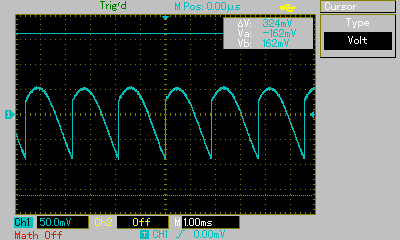
\includegraphics[width=0.95\textwidth]{content/0deg.png}
    \caption{$\Delta\phi = 0°$}
    \label{fig:0-deg}
  \end{subfigure}
  \begin{subfigure}{0.32\textwidth}
    \centering
    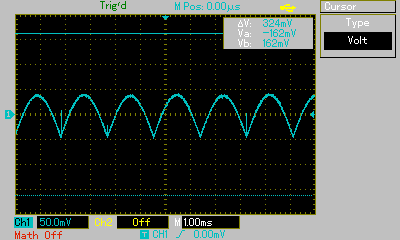
\includegraphics[width=0.95\textwidth]{content/45deg.png}
    \caption{$\Delta\phi = 45°$}
    \label{fig:45-deg}
  \end{subfigure}
  \begin{subfigure}{0.32\textwidth}
    \centering
    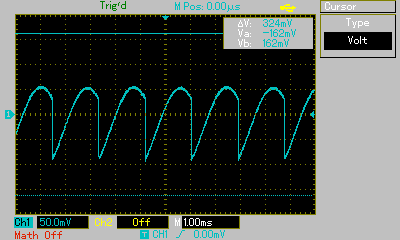
\includegraphics[width=0.95\textwidth]{content/90deg.png}
    \caption{$\Delta\phi = 90°$}
    \label{fig:90-deg}
  \end{subfigure}

  \begin{subfigure}{0.32\textwidth}
    \centering
    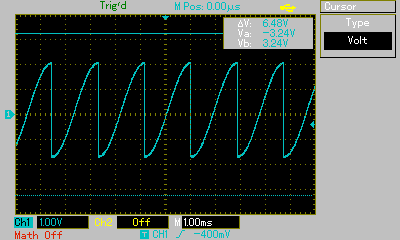
\includegraphics[width=0.95\textwidth]{content/135deg.png}
    \caption{$\Delta\phi = 135°$}
    \label{fig:135-deg}
  \end{subfigure}
  \begin{subfigure}{0.32\textwidth}
    \centering
    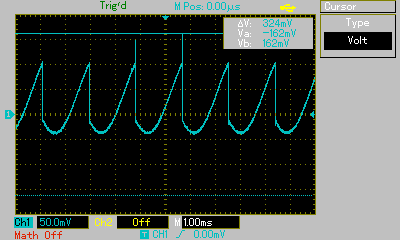
\includegraphics[width=0.95\textwidth]{content/180deg.png}
    \caption{$\Delta\phi = 180°$}
    \label{fig:180-deg}
  \end{subfigure}
  \begin{subfigure}{0.32\textwidth}
    \centering
    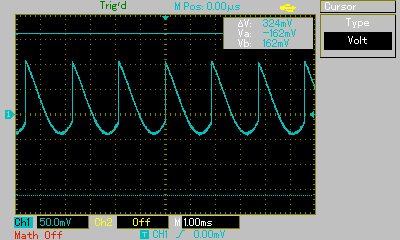
\includegraphics[width=0.95\textwidth]{content/270deg.png}
    \caption{$\Delta\phi = 270°$}
    \label{fig:270-deg}
  \end{subfigure}
  \caption{Graphen am Oszilloskop}
  \label{fig: graphen}
\end{figure}

In \autoref{fig: graphen} sind die durch den Tiefpass entstehenden Wellen bei der jeweils angegebenen Phasenverschiebung durch den Phasenverschieber. Diese Graphen entstehen durch das nicht verrauschte Signal.
Für das verrauschte Signal haben die Graphen jedoch dieselbe Form, mit der Ausnahme, dass diese an der $x$-Achse gespiegelt sind.

Die Messdaten aus \autoref{tab: Phasenverschiebung} wurden zur besseren Einsicht geplottet und es wurde ein sinusförmiger Fit über die Messwerte gelegt.
Es ist zu bemerken, dass die Werte in der Messung ohne Rauschen ein wenig kleiner waren, als jene der Messung mit Rauschen.
Die Frequenzen sind annähernd gleich, eben so wie die Phasenverschiebung zwischen $U_\text{const}$ und $U_\text{ref}$. Dies war zu erwarten, da das Rauschen durch den Lock-In-Filter größtenteils herausgefiltert wird.

\begin{figure}
  \centering
  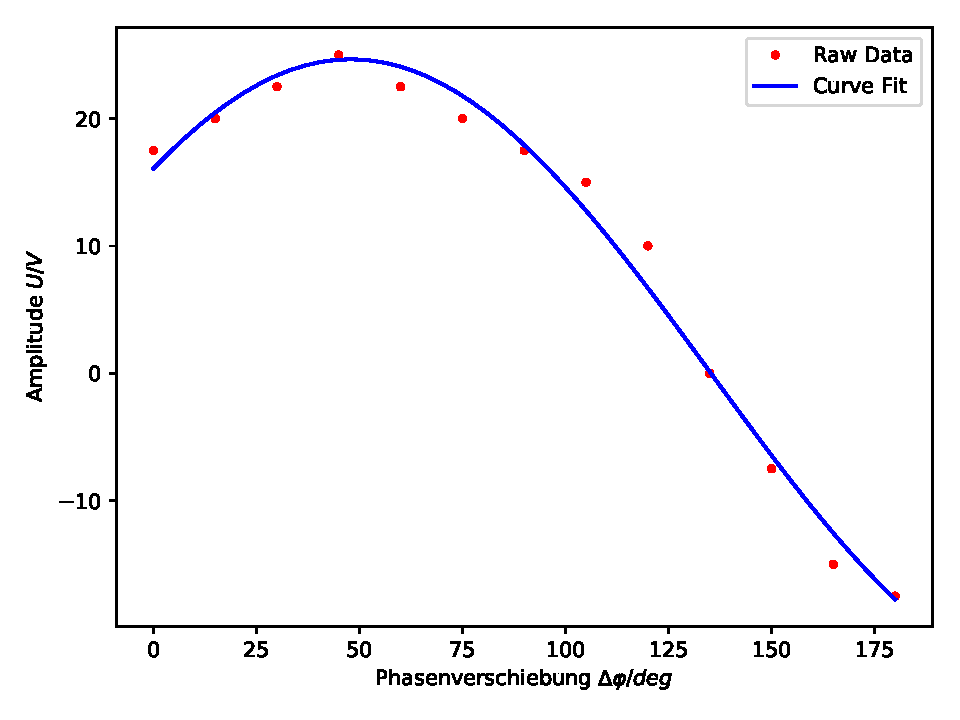
\includegraphics{plot_phase.pdf}
  \caption{Plot und Fit der Daten der Messung ohne Rauschen.}
  \label{fig:plot_phase}
\end{figure}

\begin{figure}
  \centering
  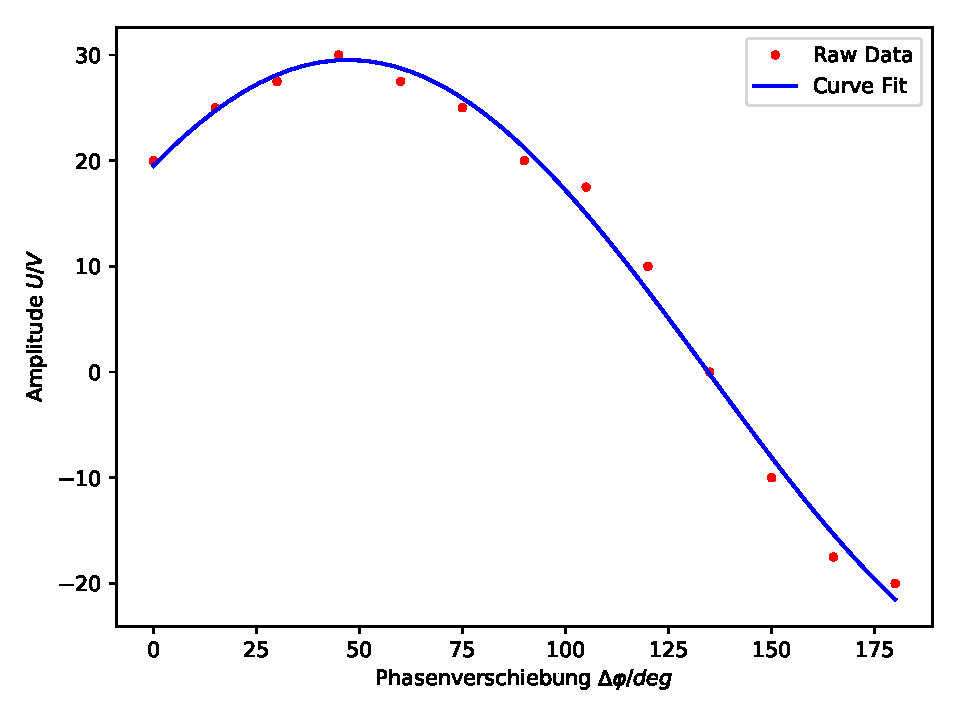
\includegraphics{plot_phase_rauschen.pdf}
  \caption{Plot und Fit der Daten der Messung mit Rauschen.}
  \label{fig:plot_phase_rauschen}
\end{figure}

Die Graphen wurden nach der Form $f(x)=a\cdot \cos(b\cdot x+c)$ geplottet. Mithilfe von Python 3.7.0 lassen sich die unverrauschten Werte als
\\ \\
\centerline{$a=(24.7 \pm 0.5)$V}
\centerline{$b=0.018 \pm 3\cdot 10^\text{-7}$}
\centerline{$c=-0.860 \pm 0.004$}
\\ \\
bestimmen. Für die verrauschten Werte ergibt sich:
\\ \\
\centerline{$a=(29.5 \pm 0.4)$V}
\centerline{$b=0.018 \pm 1.8\cdot 10^\text{-7}$}
\centerline{$c=-0.849 \pm 0.003$}

\newpage
\subsection{Messung von Lichtintensität einer LED und einer Photodiode}

Um diesen Teil korrekt auswerten zu können werden einige Einstellungen am Gerät benötigt:

\begin{table}[!htp]
  \centering
  \begin{tabular}{cccc}
    \toprule
     & \multicolumn{3}{c}{Vertärkung (Amplifier)} \\
    Frequenz / Hz & Pre-Amplifier & Lock-In & Tiefpass \\
    \midrule
    300 & 100 & 5 & 2 \\
    \bottomrule
  \end{tabular}
\end{table}

Im Folgenden wurden die Gesamtverstärkung von 1000 bereits herausgerechnet. Es konnte keine Distanz $r_\text{max}$ bestimmt werden, ab der die Photodiode keine Spannung mehr emittierte. Daher wurde die Messung bis zum durch den Messchieber begrenzten Abstand $r_\text{max}$ von $1.3$m durchgeführt.

Die Abstrahlung von einer Lichtquelle wie einer LED ist kugelförmig; daraus lässt sich die abgestrahlte Leistung als
\\ \\
\centerline{$P = I\cdot 4\pi r^2$}
\\ \\
bestimmen. So lässt sich leicht zeigen, dass für die Intensität $I$
\\ \\
\centerline{$I\sim \frac{1}{r^2}$}
\\ \\
gilt. Da die gemessene Spannung linear von der Intensität abhängt, gilt außerdem
\\ \\
\centerline{$U\sim \frac{1}{r^2}$.}
\\ \\
Die Spannung lässt sich ingesamt in Abhängigkeit von $r$ als
\\ \\
\centerline{$U(r) = \frac{a}{(r+b)^2} +c$}
\\ \\
beschreiben. Die Koeffizienten lassen sich mittels Python 3.7.0 bestimmen und sind
\\ \\
\centerline{$a=(0.182\pm 0.002)$ \!mV m²}
\centerline{$b=(0.0656\pm 0.0008)$ \!m}
\centerline{$c=(-0.080\pm 0.001)$ \!mV}
\\ \\
Das Signal wird erwartungsgemäß proportional zu $\frac{1}{r^2}$ kleiner.

\begin{table}[!htp]
  \centering
  \begin{tabular}{S[table-format=1.1] S[table-format=1.4]}
    \toprule
    {$r$ / m} & {$U_\text{LED}$ / mV} \\
    \midrule
    0.1 & 6.560 \\
    0.2 & 2.640 \\
    0.3 & 1.180 \\
    0.4 & 0.700 \\
    0.5 & 0.500 \\
    0.6 & 0.230 \\
    0.7 & 0.192 \\
    0.8 & 0.156 \\
    0.9 & 0.140 \\
    1.0 & 0.130 \\
    1.1 & 0.116 \\
    1.2 & 0.059 \\
    1.3 & 0.052 \\
    \bottomrule
  \end{tabular}
\end{table}

Die gemessenen Werte sind in \autoref{tab:intensity} zu finden. Zur Veranschaulichung wurden diese Werte in einem Plot aufgenommen und ein Fit darübergelegt. Dieser ist in \autoref{fig:plot_intensity} zu sehen.


\begin{figure}
  \centering
  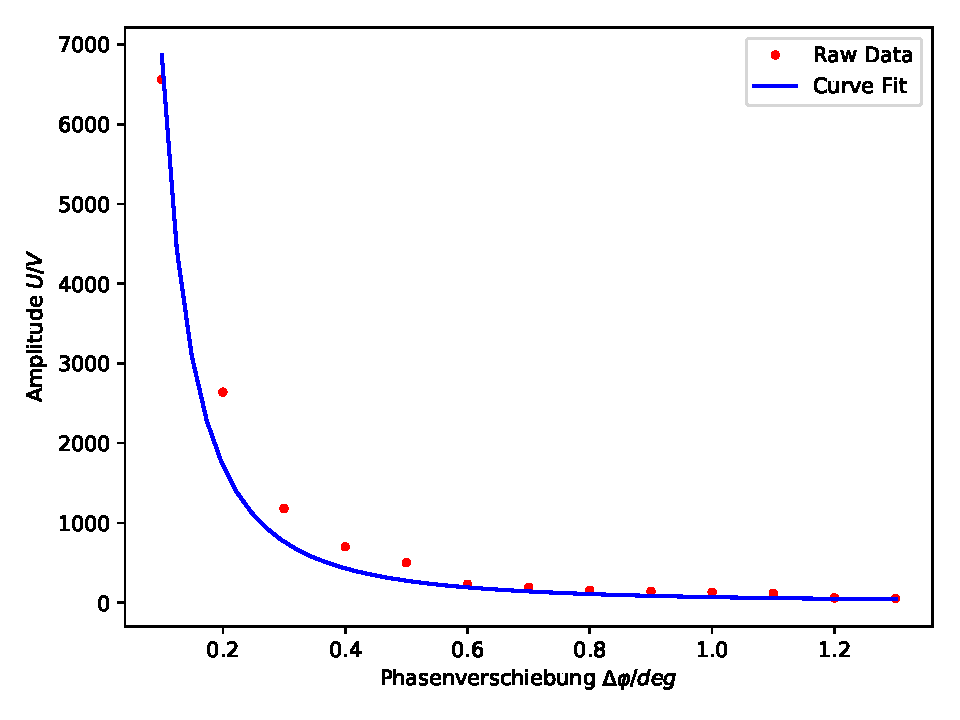
\includegraphics{plot_intensity.pdf}
  \caption{Plot und Fit der empfangen Intensität der Leuchtdiode.}
  \label{fig:plot_intensity}
\end{figure}